\documentclass[journal]{IEEEtran}

% *** CITATION PACKAGES ***
\usepackage[style=ieee]{biblatex} 
\bibliography{random_walk.bib}    %your file created using JabRef

% *** MATH PACKAGES ***
\usepackage{amsmath}

% *** PDF, URL AND HYPERLINK PACKAGES ***
\usepackage{url}
\hyphenation{op-tical net-works semi-conduc-tor}
\usepackage{graphicx}  %needed to include png, eps figures
\usepackage{float}  % used to fix location of images i.e.\begin{figure}[H]

% *** MY PACKAGES ***
\usepackage{todonotes}
\usepackage[caption=false]{subfig}

\begin{document}

% paper title
\title{Using Random Walk Simulations to Calculate Ground State Energies in Quantum Physics}

% author names 
\author{Sai Pandian, ID: 29899923}% <-this % stops a space
        
% The report headers
\markboth{PHYS6017 Computer Techniques in Physics Report 1, April 2020}
{Shell \MakeLowercase{\textit{et al.}}: Bare Demo of IEEEtran.cls for IEEE Journals}

% make the title area
\maketitle

% As a general rule, do not put math, special symbols or citations
% in the abstract or keywords.
\begin{abstract}
% Provide a summary of the session. What was done, what measurements were taken,
% brief methods, what calculations, brief conclusion.  The Abstract should be
% approximately 250 words or fewer, italicized, in 10-point Times (or Times
% Roman.) Please leave two spaces between the Abstract and the heading of your
% first section.  It should briefly summarize the essence of the paper and address
% the following areas without using specific subsection titles. Objective: Briefly
% state the problem or issue addressed, in language accessible to a general
% scientific audience. Technology or Method: Briefly summarize the technological
% innovation or method used to address the problem. Results: Provide a brief
% summary of the results and findings. Conclusions: Give brief concluding remarks
% on your outcomes. Detailed discussion of these aspects should be provided in the
% main body of the paper.
\end{abstract}

\begin{IEEEkeywords}
keywords, temperature, xxxx equation, etc.
\end{IEEEkeywords}

\section{Introduction}
% Here we have the typical use of a "W" for an initial drop letter
% and "RITE" in caps to complete the first word.
% You must have at least 2 lines in the paragraph with the drop letter
% (should never be an issue)

\IEEEPARstart{R}{andom} walks are a simple model of motion in which a path is
described as a succession of steps with each step being in a random direction on
some vector space. Random walks are useful in modelling many physical processes
that are perceived as having a pseudo-random mechanism \todo{cite}. Their
applications range from Biology to the Stock Market. This paper aims to explore
how Random Walk Simulations can be implemented to calculate the ground state
energies of different quantum systems. \todo{more}

\section{Theoretical Background}
\label{sec:TheoreticalBackground}

Random walks work descibe motion as a series of steps, with the direction of
each step being random. Figure \ref{fig:cartoon} demonstrates this concept by
considering a one-dimensional line. On this line, the ``walker'' starts at the
origin, and walks a total of 20 steps. The walker at each step has a equal
chance of stepping forwards, or stepping backwards.

\begin{figure}%[H]%[!ht]
  \begin{center}
    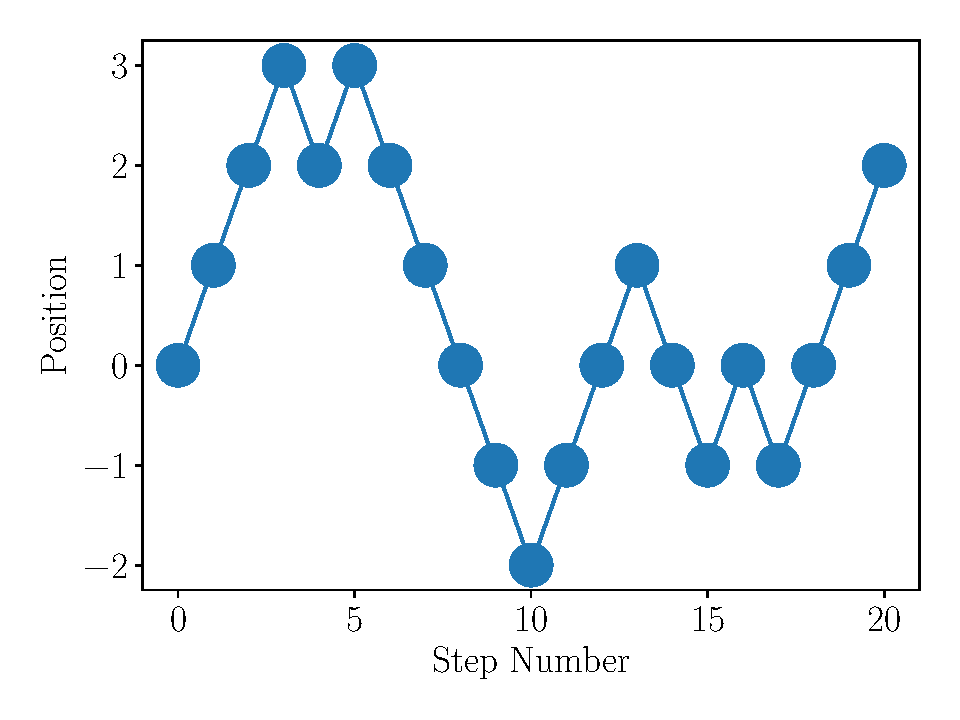
\includegraphics[width=0.45\textwidth]{images/cartoon.pdf}
    \caption{Illustrations, graphs, and photographs may fit across both columns, if necessary. Your artwork must be in place in the article.}
    \label{fig:cartoon}
  \end{center}
\end{figure}

As can be seen from the figure, it is not uncommon for the average position of
the walker to be away from the origin once the walk has concluded. This is
because the position of the walker at any step is dependent only on the position
at the previous step. If the walker happens to take a number of steps in the
same direction, it is highly unlikely for the walker to take an equal number of
steps in the opposite direction, in order to return to the origin. Thus, in such
a case, it is likely that the walker will conclude the walk in a position away
from the origin.

In this example, the walker had an equal likelihood of stepping forward or
backwards, but we can bias in one way if we want to model a particular
phenomenon. The walk is also easily extensible to multiple dimensions, as for
each extra dimension, one extra random number must be drawn. This gives a linear
increase in time-complexity, which is convenient for long computations.

Random Walk simulations can be applied to calculate the ground state energies of
Quantum Systems by solving the Schr\"{o}dinger equation \todo{cite}. Consider a
one-dimensional simple lattice system. A walker can start at a position labelled
the origin, and then proceed in a random walk. The random walk concludes after a
certain number of steps or if the walker ``dies'' on a particular step. The
probability that the walker will die is dependent on a defined potential at that
point. For example, in an infinite square well system, the potential is 0 within
a well, and infinite outside the well. So the walker will have no chance of
dying whilst inside the well, but will die if they step outside.

Let us define $p(j,n)$ as the probability that the walker will be at position
$j$ after $n$ steps and $a(j)$ as the probability that the walker will die at
position $j$. If we say:

\begin{equation}
  p(j,n) = q(j) \exp(-\lambda n)
  \label{eq:firsteq}
\end{equation}
where $q(j)$ is an arbitrary function and $\lambda$ is the rate of death, then:
\begin{equation}
  -\frac{1}{2} \frac{d^2q(j)}{dj^2} + a(j)q(j) = \lambda q(j)
  \label{eq:randomwave}
\end{equation}

The full derivation is taken from \todo{cite} and is shown in Appendix
\ref{appendix:derivation}.

Notice that Equation \ref{eq:randomwave} is in the form of a wave equation,
specifically the Schr\"{o}dinger equation:
\begin{equation}
  \label{eq:schrodinger}
  \frac{-\hbar^2}{2m}\frac{d^2 \psi}{dr^2} + V(r)\psi(r) = E\psi(r)
\end{equation}
Comparing Equation \ref{eq:randomwave} and Equation \ref{eq:schrodinger}, we can
see that the probability of death $a(j)$ is related to the potential $V(r)$,
and the rate of death $\lambda$ is related to the Energy $E$. Thus, by running
the simulation for a particular potential (i.e. rate of death), one can
determine the ground state energy of a system by calculating the rate of
death. This is the technique employed in this paper.

\section{Method}

The Random Walk is implemented computationally \todo{cite} and is extensible
to multiple dimensions. For a $N$-dimensional lattice, at each point there are
$2N$ possible directions for the walker to move. So a direction is selected
randomly using a Mersenne Twister pseudorandom number generator (pRNG). This algorithm
was chosen as it is a very fast implementation of a pRNG \todo{cite} and it
passes many statistical randomness tests \todo{cite}, having a very large
period of $2^{19937-1}$.

The random walk ends when a walker dies, with a
specifically chosen $a(j)$. Initially, the $a(j)$ is chosen to be that of an
infinite square well \todo{cite}, that is:
\begin{equation}
  \label{eq:squarewell}
    a(j) =
    \begin{cases}
      0,& \text{if } j < J\\
      \infty,& \text{if } j \geq J
    \end{cases}
    \nonumber
\end{equation}
where J is a well-defined boundary. So the walker has no chance of dying whilst
within the well, but will die immediately once reaching the boundary. As
explained in Section \ref{sec:TheoreticalBackground}, we expect that given
sufficient time, all the walkers will reach the boundary and die. But in order
to save computational resources, a maximum number of steps may also be defined,
such that a walker will also die should they move that number of steps without
reaching a boundary. This was not initially implemented, as it can introduce
systemic errors, since there would be a disproportionate number of walkers dying
on the maximum number of steps.

Thus, the Schr\"{o}dinger equation inside a one-dimensional infinite square well
is simply that of a free particle \todo{cite}:
\begin{equation}
  \frac{-\hbar^2}{2m}\frac{d^2 \psi}{dx^2} = E\psi(x)
  \nonumber
\end{equation}
where $x$ is the position of the walker. By making the substitution $x = J
\times j/R$, such that $j=R$ corresponds to the walker being at the boundary, we
obtain:
\begin{equation}
  \begin{split}
    -\frac{\hbar^2}{2m}\frac{R^2}{J^2}\frac{d^2\psi}{dj^2} &= E\psi(x)\\
    -\frac{1}{2}\frac{d^2\psi}{dj^2} &= \frac{mJ^2E}{\hbar^2R^2}\psi(x)
  \end{split}
  \nonumber
\end{equation}

If we compare this to Equation \ref{eq:randomwave}, allowing $a(j) = 0$, we see
that:
\begin{equation}
  \begin{split}
    \lambda &= \frac{mJ^2E}{\hbar^2R^2} \\
    E &= \lambda R^2 \frac{\hbar^2}{mJ^2}
  \end{split}
  \nonumber
\end{equation}

So, by calculating the death rate $\lambda$, we can find the ground state energy
of a particle in an infinite square well.

But the known ground state of a particle in an infinite square well is
$\frac{\pi^2}{8}\frac{\hbar^2}{mJ^2}$ \todo{cite}. This implies that we expect $\lambda
R^2=\frac{\pi^2}{8}$ where R is the boundary of the well. Thus, we expect to
find a $\lambda$ that is close to this theoretical value.


To find the rate of death $\lambda$, we consider Equation \ref{eq:firsteq}. With
some simple manipulation:
\begin{equation}
  \begin{split}
    p(j, n) & = q(j) \exp(-\lambda n)\\
    \log(p) & = \log(q \exp(-\lambda n)) \\
    \log(p) & = -\lambda n + log(q)
  \end{split}
  \nonumber
\end{equation}
Thus, by plotting the logarithm of the probability of surviving $n$ steps
against the number of steps $n$, we can obtain the death rate $\lambda$ from the
gradient.

Varying the boundary $J$ of the square well will affect the accuracy of the
final answer, and this is also investigated here.


\section{Results and Discussion}



\begin{figure*}[ht!]
  \centering
  \subfloat[Histogram of probability of dying on particlar step]
  {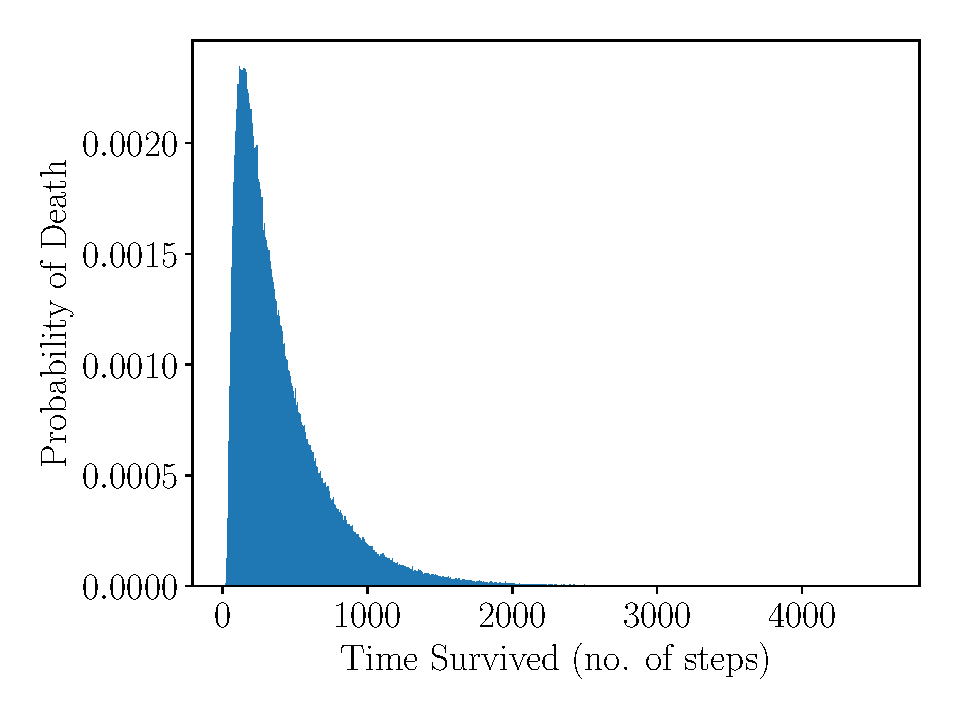
\includegraphics[width=0.5\textwidth]{images/exp_plot.pdf}
  \label{fig:hist}}
  \centering
  \subfloat[Histogram of probability of dying on particular step in a logarithmic scale]
  {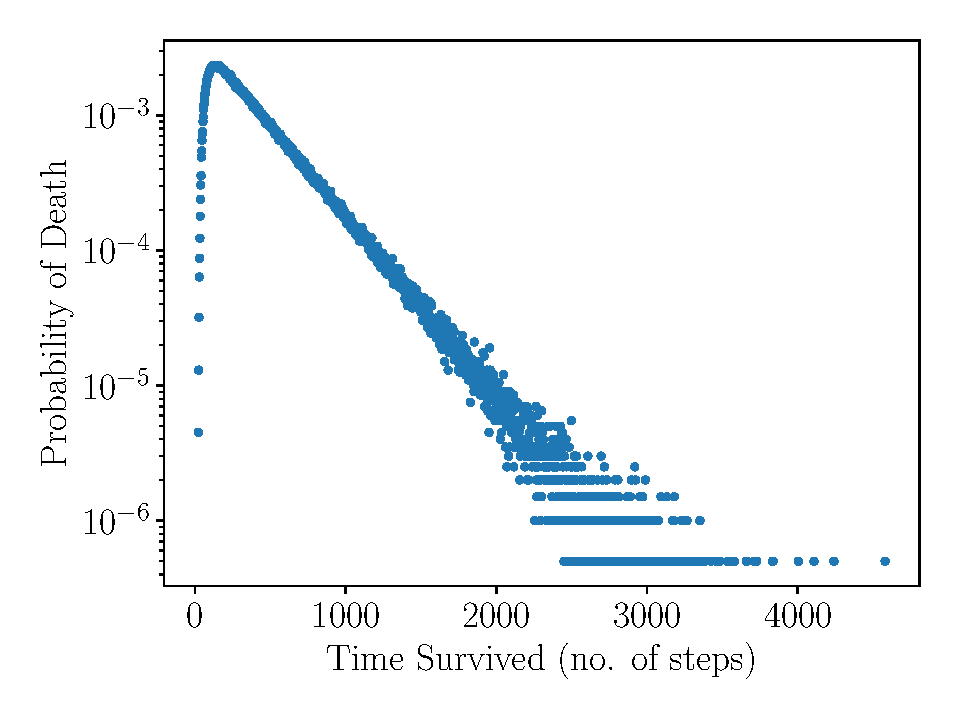
\includegraphics[width=0.5\textwidth]{images/line_plot.pdf}
    \label{fig:loghist}}
  \caption{Histograms showing the Probability of dying on a particular step in
    an infinite square well with $J = 20$. As can be seen, the peak is away from the
    origin, as is expected since it is not likely for a walker to die on a step $n$
    where $n < J$. The exponential decay after the peak is evident, implying a
    straight line shape if plotted on a logarithmic scale, which can be seen on
    the right hand side plot. In this logarithmic scale plot, the peak being away
    from the origin is clearer.}
  \label{fig:expplots}
\end{figure*}



\begin{figure*}[ht!]
  \centering
  \subfloat[Histogram of probability of surviving to at least a particlar step]
  {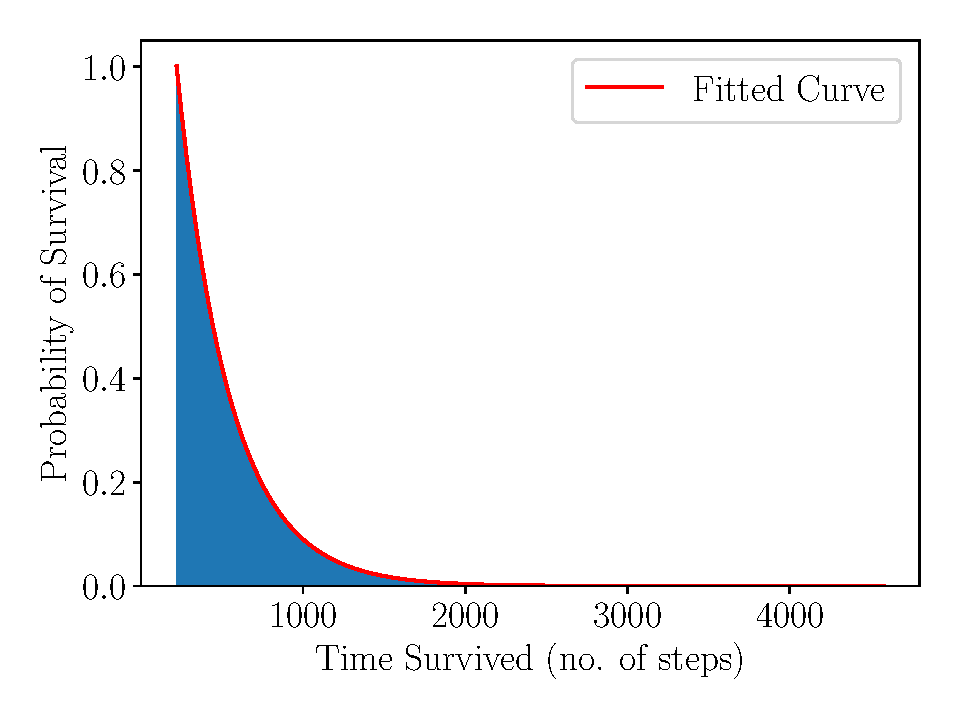
\includegraphics[width=0.5\textwidth]{images/cum_exp_plot.pdf}
  \label{fig:cumhist}}
  \centering
  \subfloat[Histogram of probability of surviving to at least a particular step
  in a logarithmic scale]
  {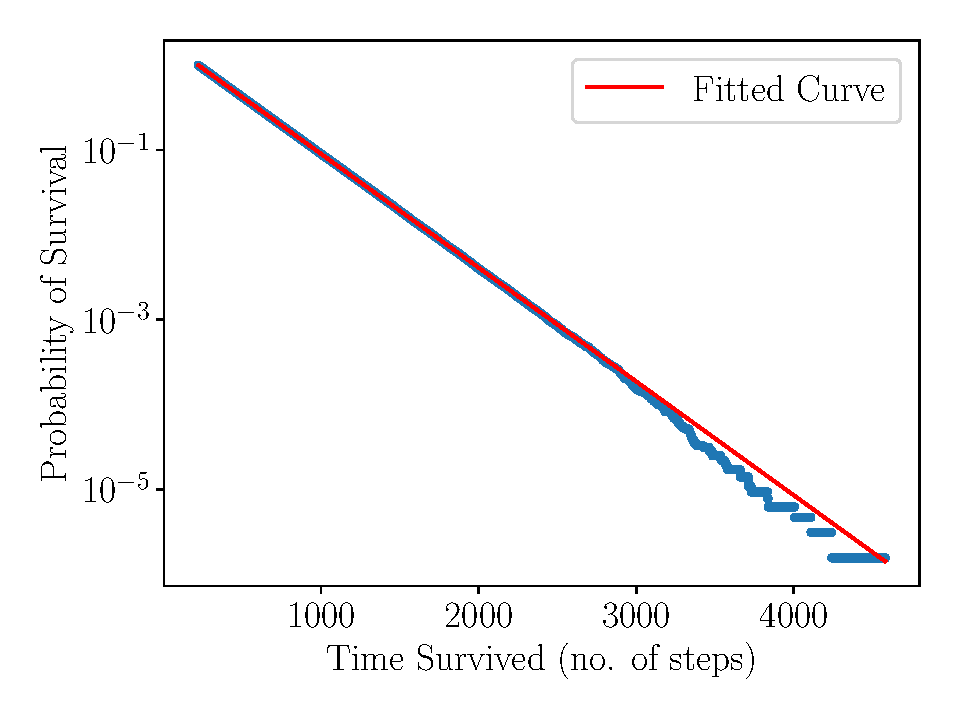
\includegraphics[width=0.5\textwidth]{images/cum_line_plot.pdf}
  \label{fig:cumloghist}}
  \caption{Histogram showing the Probability of surviving to at least a
      particular step in an infinite square well with $J = 20$. This is a
      cumulative sum of the bins in Figure \ref{fig:hist}. As can be seen, the
      peak is at the origin, since it is certain that no walker will die on the
      first step. An exponential decay curve provides a good fit, with an $R^2$
      value of 0.9999998, very close to 1. Plotting on a logarithmic scale shows
      the straight line fit, the gradient of which is $\lambda$, giving $\lambda
      J^2 = 1.2334$, with a negligible error.}
  \label{fig:cumplots}
\end{figure*}


\begin{figure}[!ht]
  \begin{center}
    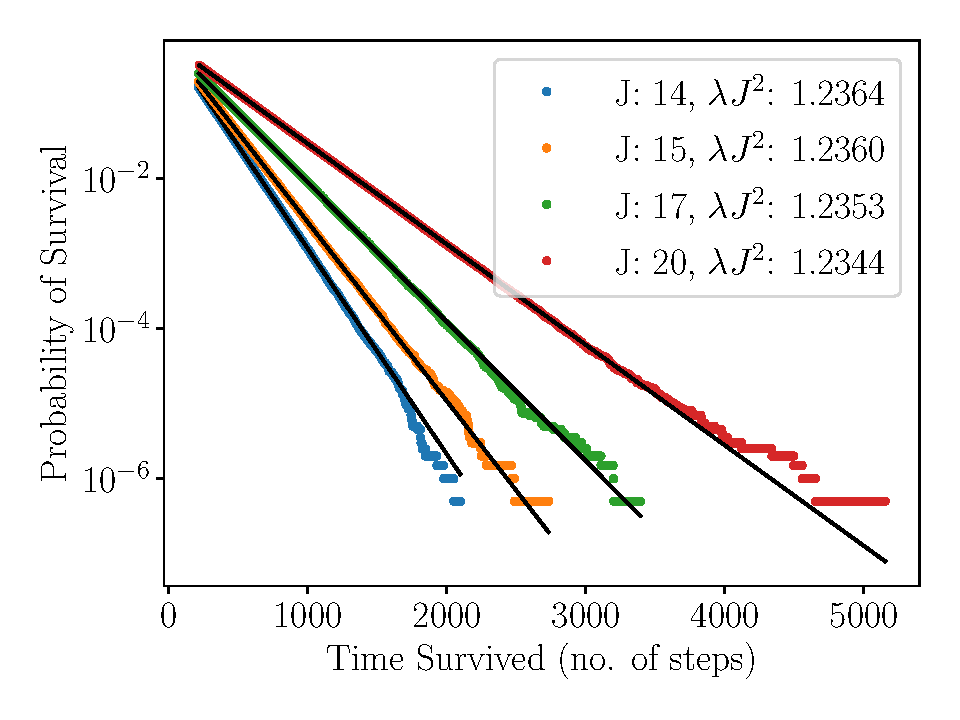
\includegraphics[width=0.45\textwidth]{images/multiplot.pdf}
    \caption{Histogram plotted on a logarithmic scale showing the Probability of
      surviving to at least a particualr step in different infinite square wells with
      different boundaries $J$. The $\lambda J^2$ values for each are shown. The
      values get closer to the theoretical value of $\frac{\pi^2}{8}$ as we increase
      the size of the well. This is likely due to more walkers surviving to a higher
      number of steps, as the well size is increased.}
    \label{fig:multi_line_plot}
  \end{center}
\end{figure}


\begin{figure}[!ht]
  \begin{center}
    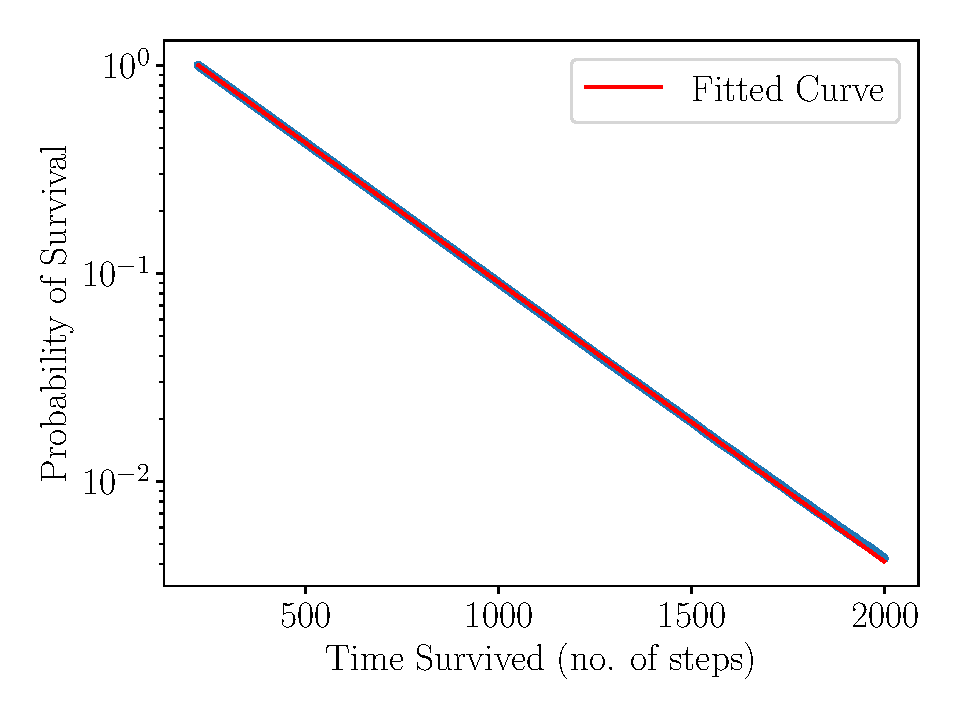
\includegraphics[width=0.45\textwidth]{images/cum_line_plot_cutoff.pdf}
    \caption{Histogram plotted on a logarithmic scale showing the Probability of
      surviving to at least a particular step in an infinite square well with $J
      = 20$, and also introducing a maximum number of steps at 2000, after which
      all walkers will die. This saves computational resources but introduces
      some systematic error, as there will now be a disproportionately high
      number of walkers in the 2000 steps bin.}
    \label{fig:cum_line_cutoff_plot}
  \end{center}
\end{figure}

\section{Conclusions}

Sample Text


% if have a single appendix:
%\appendix[Proof of the Zonklar Equations]
% or
%\appendix  % for no appendix heading
% do not use \section anymore after \appendix, only \section*
% is possibly needed

% use appendices with more than one appendix
% then use \section to start each appendix
% you must declare a \section before using any
% \subsection or using \label (\appendices by itself
% starts a section numbered zero.)
%



\appendices
\section{Random Walk Schr\"{o}dinger Equation Derivation}
\label{appendix:derivation}
Let us denote the probability that the walker is at position $j$ after $n$ steps
as $p(j,n)$ and the probabilty that the walker will die at position $j$ as
$a(j)$. We will denote the position-step number coordinates as $[j, n]$. Thus,
for a walker to have coordinates $[j, n+1]$, in the previous step, they must have
had coordinates $[j \pm 1, n]$. So we can say:

\begin{equation}
  \label{eq:probability}
  p(j, n+1) =  \frac{1}{2}(1-a(j))(p(j-1,n) + p(j+1,n))
\end{equation}

If $a(j)$ is small and $n$ is large, then we can say $p(j, n)$ is a continuous
function and we can use Taylor expansion to expand each of $p(j+1, n)$,
$p(j-1,n)$, and $p(j, n+1)$:

\begin{equation}
  p(j+1, n) = p(j,n) + \frac{\partial p}{\partial j} + \frac{1}{2}
  \frac{\partial^2 p}{\partial j^2} + ...
  \nonumber
\end{equation}
\begin{equation}
  p(j-1, n) = p(j,n) - \frac{\partial p}{\partial j} + \frac{1}{2}
  \frac{\partial^2 p}{+\partial j^2} + ...
  \nonumber
\end{equation}
\begin{equation}
  p(j, n+1) = p(j, n) + \frac{\partial p}{\partial n} + ...
  \nonumber
\end{equation}

We can now substitute these expansions into Equation \ref{eq:probability}, we
find:

\begin{equation}
  p(j, n) + \frac{\partial p}{\partial n} = (1-a(j))\Big(p +
  \frac{1}{2}\frac{\partial^2 p}{\partial j^2}\Big)
  \nonumber
\end{equation}

But the probability of death $a(j)$ and the second derivative are so small, that
their product is neglected. We also let $p(j,n) = q(j) \exp(-\lambda n)$ so that:

\begin{equation}
  -\frac{1}{2} \frac{d^2q(j)}{dj^2} + a(j)q(j) = \lambda q(j)
  \nonumber
\end{equation}

\printbibliography

\end{document}


